\documentclass{article}
\usepackage{fontspec}
\usepackage{graphicx}
\usepackage{amssymb}
\usepackage{wasysym}
\usepackage{enumitem}
\usepackage{fontawesome5}
\usepackage{xcolor}
\usepackage{comment}

\usepackage[margin=1.5cm]{geometry}

\newcommand{\playbookTitle}{}

\newcommand{\playbookImage}{}

\newcommand{\flavorText}{}

\newcommand{\charNames}{}

\newcommand{\charAnimals}{}

\newcommand{\charEnhancementOne}{}
\newcommand{\charEnhancementTwo}{}
\newcommand{\charEnhancementThree}{}
\newcommand{\charEnhancementFour}{}
\newcommand{\charEnhancementFive}{}
\newcommand{\charEnhancementSix}{}

\newcommand{\moveOne}{}
\newcommand{\moveTwo}{}
\newcommand{\moveThree}{}
\newcommand{\moveFour}{}
\newcommand{\moveFive}{}

\newcommand{\relationsOne}{}
\newcommand{\relationsTwo}{}
\newcommand{\relationsThree}{}

\newcommand{\leadingPrinciplesOne}{}
\newcommand{\leadingPrinciplesTwo}{}
\newcommand{\leadingPrinciplesThree}{}
\newcommand{\leadingPrinciplesFour}{}

\newcommand{\flipsideOne}{}
\newcommand{\flipsideTwo}{}
\newcommand{\flipsideThree}{}
\newcommand{\flipsideFour}{}

\setmainfont{Arial}
\parindent0mm
\linespread{1.2}

\begin{document}
\pagenumbering{gobble}

\vspace*{\fill}

\begin{figure}[tph!]
\centering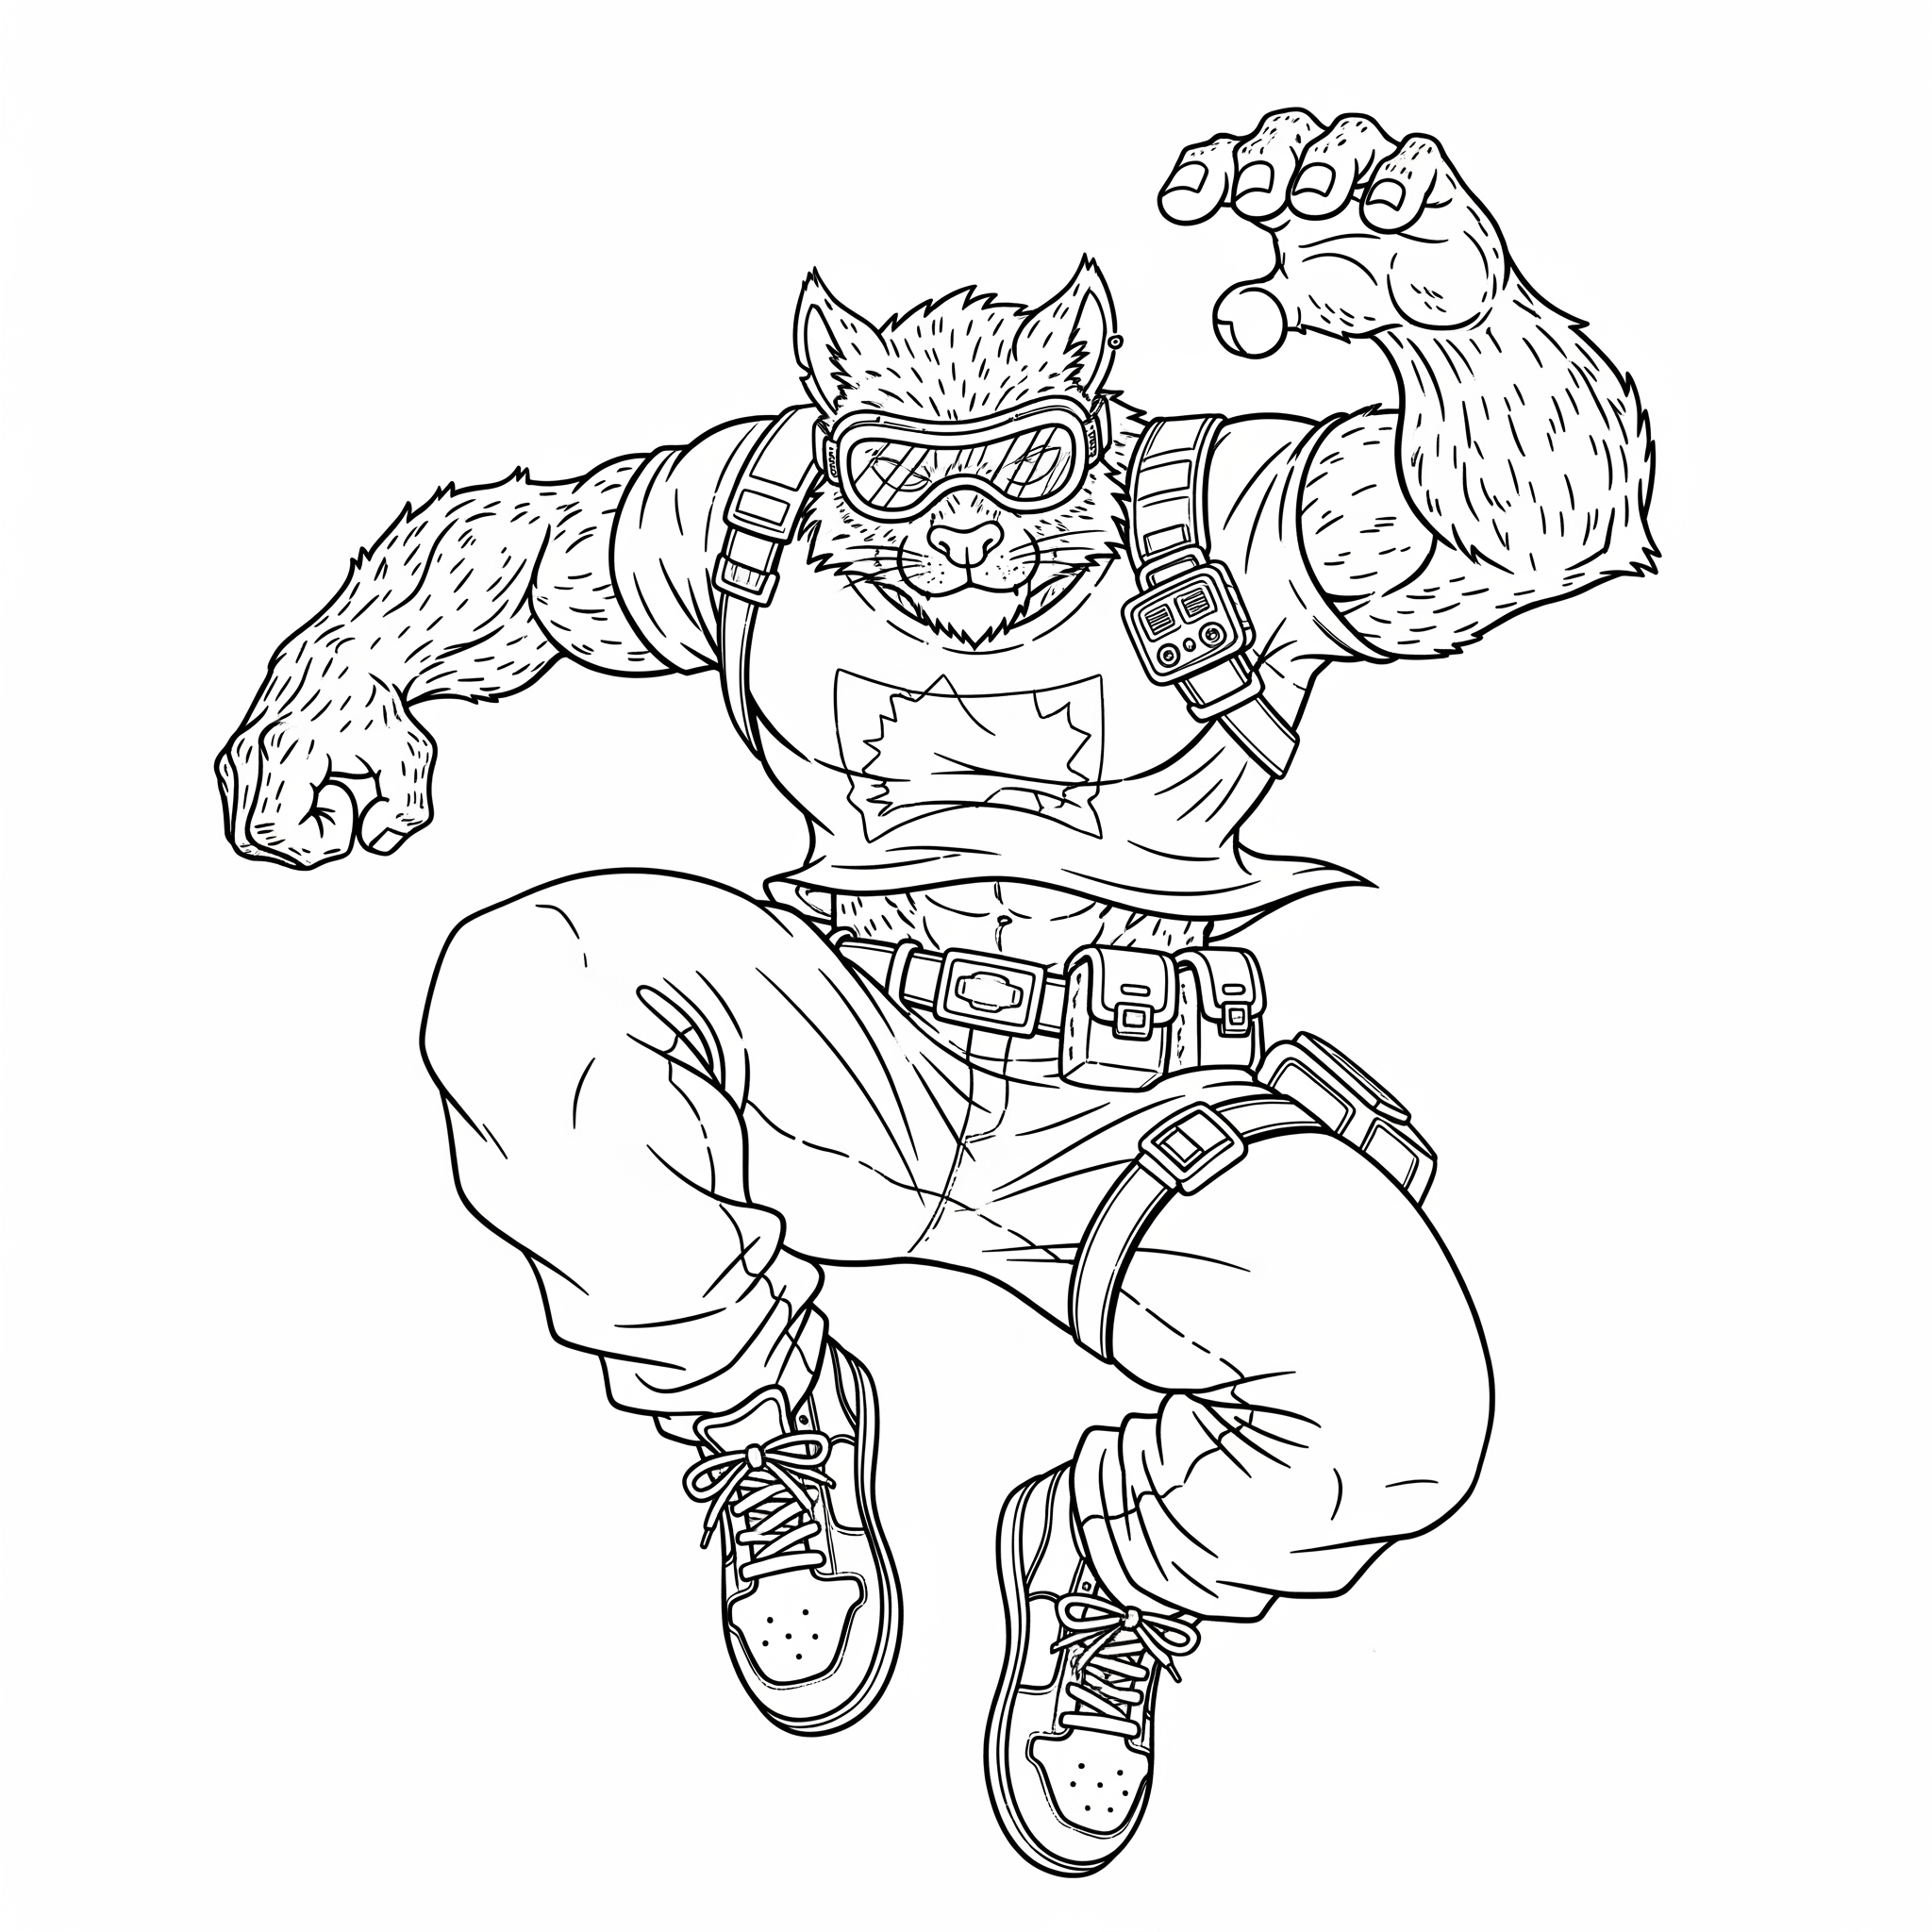
\includegraphics[width=12cm]{images/frontCover.png}
\end{figure}
\centering\Huge\fontspec{TradeWinds-Regular.ttf}Martial Mutant Misfitz!

\newpage
\pagenumbering{arabic}
\raggedright
\section*{\fontspec{TradeWinds-Regular.ttf}What is Martial Mutant Misfitz?}
\normalfont\large You are humanoid animal mutants. Human society rejects you. Your appearance is alien and off-putting to most humans. Fortunately, a mentor came into your life. Taking care of you when you needed it the most. Training you in martial prowess, and teaching you how to leverage your new abilities. A mentor hiding your from society and shielding you from harm. But this could soon end, as a new evil rises, that threatens the city. Who is gonna stop it? Who if not you?!

Martial Mutant Misfitz is a game about whacky teenagers mutated into animals. It's a game about stylish fighting and kung fu. It also is a game about being an outsider --- he feeling of not fitting into society. And lastly, it's a game about family.
\newpage

\begin{comment}
\renewcommand{\playbookTitle}{Aberrant}

\renewcommand{\playbookImage}{images/aberrant.png}

\renewcommand{\flavorText}{
\textit{Literally a freak of nature. Or rather science... }\\
\medskip
You mutated a bit too far. Your once beautiful face and body is now hideous. We're talking spikes, ooze, hunchback, you got the whole program. It's unthinkable that you go near human society. On the flipside, you received some crazy powers...\\
\medskip
You often need special attention and care. May it be the amount of food you consume, to find clothes in your size or that you crushed something by accident... again.
}

\renewcommand{\charNames}{1.Crux, 2.Maw, 3.Slitha, 4.Acida, 5.Scabarella, 6.Gnarl, \rule{2cm}{1pt}}

\renewcommand{\charAnimals}{1.Shark, 2.Worm, 3.Vulture, 4.Spider, 5.Crab, 6.Octopus, \rule{2cm}{1pt}}

\renewcommand{\charEnhancementOne}{\textbf{Razorsharp Spikes} (2 harm, hand, sharp)}
\renewcommand{\charEnhancementTwo}{\textbf{Extra limbs} (Once per scene, roll twice on \emph{Kick Ass!})}
\renewcommand{\charEnhancementThree}{\textbf{Back-Mounted Chemical Feed} (+1 Grit)}
\renewcommand{\charEnhancementFour}{\textbf{Rocklike Skin} (1 armor)}
\renewcommand{\charEnhancementFive}{\textbf{Hyper-Acid Digestion Track} (You can eat and digest everything.)}
\renewcommand{\charEnhancementSix}{\textbf{Amphibian Lung Gills}  (Can breath in and out of water, probably even more fluids.)}
%vertebrae whip 2 harm close

\renewcommand{\moveOne}{\textbf{It's not a glitch --- it's a feature.} Your mutation is unstable. Choose one of your enhancements and roll +Grit. On a 10+, exchange the chosen enhancement with another \playbookTitle enhancement. On a 7-9, roll for the new enhancement.}
\renewcommand{\moveTwo}{\textbf{This will just sting a little.} When you spend some time with a living or dead enemy, you can read their memories. Roll +Discipline. On a 7-9, ask the GM one of the following questions, on a 10+ two.
\vspace{-6pt}
\begin{itemize}
    \setlength\itemsep{-0.5em}
    \item Who do they work for?
    \item Where do they live?
    \item What is their favourite food?
    \item What was their childhood like?
    \item Do they have loved ones?
\end{itemize}}
\renewcommand{\moveThree}{\textbf{Walls are optional.} When you break through walls, destroy or throw obstacles. Roll +Grit. On a hit, choose one of the following:
\vspace{-6pt}
\begin{itemize}
    \setlength\itemsep{-0.5em}
\item Deal 2 harm
\item Deal 1 harm, area
\item Get or give +1 forward
\item You draw attention - enemies focus on you.
\item You create a advantageous position for your team.
\item You create a new "shortcut"
\end{itemize}
\vspace{-6pt}
On a 7-9 additionally choose one of the following, according to the narrative:
\vspace{-6pt}
\begin{itemize}
    \setlength\itemsep{-0.5em}
\item  Take 1 harm
\item  Take 1 condition
\item  Decrease the Team Mojo by 1
\end{itemize}

}
\renewcommand{\moveFour}{\textbf{Beauty's overrated. I went for memorable.} If a non hostile sees you for the first time, roll +Grit. On a hit choose one: They are stunned, afraid or fascinated. On a 7-9 they additionally react poorly.}
\renewcommand{\moveFive}{\textbf{Here, take some of my chemicals. They make you strong.} When you give some of your stabilizing chemicals to an ally, roll +Style. On a hit, they get +1 forward. On a 7-9 they additionally become poisoned.}

\renewcommand{\relationsOne}{\rule{2cm}{1pt} accidently used some of your stabilization chemicals. Ask the player how it came to this. Explain what temporary effect they had on them.}
\renewcommand{\relationsTwo}{You broke something dear of \rule{2cm}{1pt}. Ask the player what it was.}
\renewcommand{\relationsThree}{You and \rule{2cm}{1pt} share an absolutely weird hobby. What is it?}

\renewcommand{\leadingPrinciplesOne}{Need special treatment}
\renewcommand{\leadingPrinciplesTwo}{Your mutations behave weirdly}
\renewcommand{\leadingPrinciplesThree}{Mutate in weird ways}
\renewcommand{\leadingPrinciplesFour}{Don't fit}

\renewcommand{\flipsideOne}{Create problems}
\renewcommand{\flipsideTwo}{Draw attention}
\renewcommand{\flipsideThree}{Break something}
\renewcommand{\flipsideFour}{Feel left alone}

\pagenumbering{gobble}

\vspace*{\fill}

\begin{figure}[h!]
\centering\includegraphics[width=12cm]{\playbookImage}
\vspace{-\baselineskip}\vspace{+0.1pt}
\rule{\linewidth}{2pt}
\end{figure}
\Huge\fontspec{TradeWinds-Regular.ttf}The \playbookTitle

\normalfont\large
\medskip

\flavorText

\newpage

\Large\fontspec{TradeWinds-Regular.ttf}Animal

\medskip

\normalfont\large \charAnimals

\medskip

\Large\fontspec{TradeWinds-Regular.ttf}Names

\medskip

\normalfont\large \charNames

\medskip

\Large\fontspec{TradeWinds-Regular.ttf}Enhancements

\medskip

\normalfont\large Pick or roll two:

\(\square\) \charEnhancementOne

\(\square\) \charEnhancementTwo

\(\square\) \charEnhancementThree

\(\square\) \charEnhancementFour

\(\square\) \charEnhancementFive

\(\square\) \charEnhancementSix

\medskip

\Large\fontspec{TradeWinds-Regular.ttf}Advancements \(\LARGE \Circle \Circle \Circle \Circle \Circle \)

\medskip

\normalfont\large

\begin{tabular}{l @{\hspace{2cm}} l}
\(\square\) Get +1 Power, max +3 & \(\square\) Take another \playbookTitle~move \\
\(\square\) Get +1 Cool, max +3 & \(\square\) Take another \playbookTitle~enhancement \\
\(\square\) Get +1 Wits, max +3 & \(\square\) Take a move from another playbook \\
\(\square\) Get +1 Heart, max +3 & \(\square\) Take a move from another playbook \\
\(\square\) Get +1 Weird, max +3 & \\
\end{tabular}

\medskip

\Large\fontspec{TradeWinds-Regular.ttf}Conditions

\medskip

\normalfont\large

\(\square\) \textbf{Exposed} (-2 to Power until you eliminate or evade the skeptical)\\
\(\square\) \textbf{Angry} (-2 to Cool until you hurt someone or break something)\\
\(\square\) \textbf{Stressed} (-2 to Weird until you say sth hurtful to someone)\\
\(\square\) \textbf{Jealous} (-2 to Heart until you go on an ego trip)\\
\(\square\) \textbf{Insecure} (-2 to Charm until you take a comment to wrong way)\\
\(\square\) \textbf{Poisoned}  (-1 to all stats until healed)

\medskip

\Large\fontspec{TradeWinds-Regular.ttf}Harm \(\bigtriangledown \bigtriangledown \bigtriangledown \bigtriangledown | \bigtriangledown \bigtriangledown\)

\medskip

\Large\fontspec{TradeWinds-Regular.ttf}Stats

\normalfont\Huge

%Add tabular?
\faBomb~\textcolor{lightgray}{\faCircle[regular]} \hspace{0.5cm} \faStar~\textcolor{lightgray}{\faCircle[regular]} \hspace{0.5cm} \faHeart~\textcolor{lightgray}{\faCircle[regular]} \hspace{0.5cm} \faBrain~\textcolor{lightgray}{\faCircle[regular]} \hspace{0.5cm} \faPizzaSlice~\textcolor{lightgray}{\faCircle[regular]}

\medskip

\Large\fontspec{TradeWinds-Regular.ttf}Notes

\newpage

\Large\fontspec{TradeWinds-Regular.ttf}\playbookTitle~Moves

\medskip

\normalfont\large

\begin{itemize}[label=$\square$]

\item \moveOne

\item \moveTwo

\item \moveThree

\item \moveFour

\item \moveFive

\end{itemize}


\Large\fontspec{TradeWinds-Regular.ttf}Relations

\medskip

\normalfont\large

\begin{itemize}[label=$\square$]
    \item \relationsOne
    \item \relationsTwo
    \item \relationsThree
\end{itemize}

\begin{tabular}{l @{\hspace{2cm}} l}

\Large\fontspec{TradeWinds-Regular.ttf}Leading Principles & \Large\fontspec{TradeWinds-Regular.ttf}Flipside \\

\normalfont\large

$\bullet$ \leadingPrinciplesOne & $\bullet$ \flipsideOne \\
$\bullet$ \leadingPrinciplesTwo &  $\bullet$ \flipsideTwo \\
$\bullet$ \leadingPrinciplesThree &  $\bullet$ \flipsideThree \\
$\bullet$ \leadingPrinciplesFour &  $\bullet$ \flipsideFour \\

\end{tabular}

\newpage
\renewcommand{\playbookTitle}{Brainiac}

\renewcommand{\playbookImage}{images/brainiac.png}

\renewcommand{\flavorText}{
\textit{"For every problem there is a solution and I will find it."}\\
\medskip
You love science and solving puzzles. You are the brains of your team.\\
\medskip
Towards the others you often pled for waiting to receive more data, diskussing and analyzing.
}

\renewcommand{\charNames}{1.Cypher, 2.Echo, 3.Vector, 4.Ivy, 5.Pixel, 6.Glitch, \rule{2cm}{1pt}}

\renewcommand{\charAnimals}{1.Octopus, 2.Raven, 3.Owl, 4.Dolphin, 5.Fox, 6.Gorilla, \rule{2cm}{1pt}}

\renewcommand{\charEnhancementOne}{\textbf{MutaTech Mark IV Attack Drones} (1 harm, far)}
\renewcommand{\charEnhancementTwo}{\textbf{Backpack-Lab} Gives you the opportunity to analyze and synthesize chemicals on the go.}
\renewcommand{\charEnhancementThree}{\textbf{MorphSwarm Units} (1 harm, hand, choose blunt, piercing, …)}
\renewcommand{\charEnhancementFour}{\textbf{Hyper-Cognition} (choose one additional move)}
\renewcommand{\charEnhancementFive}{\textbf{Ultra-Adaptive NeuroShield} (1 armor)}
\renewcommand{\charEnhancementSix}{\textbf{EMP} (1 harm vs. mechanical, area)}

\renewcommand{\moveOne}{\textbf{This won’t take long.} Hack, repair or manipulate something. Roll +Wits. On a hit you surpass the challenge. On a 7-9 you only get a limited time in the system.}
\renewcommand{\moveTwo}{
You can’t hide from thermals. Roll +Wits. On a 10+, ask the GM two of the following questions, on a 7-9 one.
\begin{itemize}
    \item Is there someone behind this wall?
    \item What would someone see if the visibility was better?
    \item How many individuals are we dealing with?
    \item What is a weak spot here?
    \item How do we get in or out?
    \item What is the safest way forward?
    \item What is some valuable piece of information?
\end{itemize}
}
\renewcommand{\moveThree}{\textbf{Hope they backed this up.} When you receive information or hack into a system, you get or give +1 forward.}
\renewcommand{\moveFour}{\textbf{Crafted with love... and a little bit of panic.} Roll +Weird. On a hit you improvise a weapon (1 harm) and get +1 forward. On a 7-9 it only lasts for this combat.}
\renewcommand{\moveFive}{\textbf{Keep calm and pretend this is fine.} Roll +Weird. On a hit you clear a condition off of you}

\renewcommand{\relationsOne}{\rule{2cm}{1pt} and I love the same video game. How is it called? What is it about?}
\renewcommand{\relationsTwo}{I taught \rule{2cm}{1pt} about the science field I love. What is it?}
\renewcommand{\relationsThree}{I found unusual data or browser history from \rule{2cm}{1pt} on the shared computer. Ask the player what it was about.}

\renewcommand{\leadingPrinciplesOne}{Be the rationale}
\renewcommand{\leadingPrinciplesTwo}{Solve puzzles}
\renewcommand{\leadingPrinciplesThree}{Provide information}
\renewcommand{\leadingPrinciplesFour}{Correct wrong or imprecise information}

\renewcommand{\flipsideOne}{Think too long}
\renewcommand{\flipsideTwo}{Don't act}
\renewcommand{\flipsideThree}{Be hesitant}
\renewcommand{\flipsideFour}{Have troubles deciding}

\pagenumbering{gobble}

\vspace*{\fill}

\begin{figure}[h!]
\centering\includegraphics[width=12cm]{\playbookImage}
\vspace{-\baselineskip}\vspace{+0.1pt}
\rule{\linewidth}{2pt}
\end{figure}
\Huge\fontspec{TradeWinds-Regular.ttf}The \playbookTitle

\normalfont\large
\medskip

\flavorText

\newpage

\Large\fontspec{TradeWinds-Regular.ttf}Animal

\medskip

\normalfont\large \charAnimals

\medskip

\Large\fontspec{TradeWinds-Regular.ttf}Names

\medskip

\normalfont\large \charNames

\medskip

\Large\fontspec{TradeWinds-Regular.ttf}Enhancements

\medskip

\normalfont\large Pick or roll two:

\(\square\) \charEnhancementOne

\(\square\) \charEnhancementTwo

\(\square\) \charEnhancementThree

\(\square\) \charEnhancementFour

\(\square\) \charEnhancementFive

\(\square\) \charEnhancementSix

\medskip

\Large\fontspec{TradeWinds-Regular.ttf}Advancements \(\LARGE \Circle \Circle \Circle \Circle \Circle \)

\medskip

\normalfont\large

\begin{tabular}{l @{\hspace{2cm}} l}
\(\square\) Get +1 Power, max +3 & \(\square\) Take another \playbookTitle~move \\
\(\square\) Get +1 Cool, max +3 & \(\square\) Take another \playbookTitle~enhancement \\
\(\square\) Get +1 Wits, max +3 & \(\square\) Take a move from another playbook \\
\(\square\) Get +1 Heart, max +3 & \(\square\) Take a move from another playbook \\
\(\square\) Get +1 Weird, max +3 & \\
\end{tabular}

\medskip

\Large\fontspec{TradeWinds-Regular.ttf}Conditions

\medskip

\normalfont\large

\(\square\) \textbf{Exposed} (-2 to Power until you eliminate or evade the skeptical)\\
\(\square\) \textbf{Angry} (-2 to Cool until you hurt someone or break something)\\
\(\square\) \textbf{Stressed} (-2 to Weird until you say sth hurtful to someone)\\
\(\square\) \textbf{Jealous} (-2 to Heart until you go on an ego trip)\\
\(\square\) \textbf{Insecure} (-2 to Charm until you take a comment to wrong way)\\
\(\square\) \textbf{Poisoned}  (-1 to all stats until healed)

\medskip

\Large\fontspec{TradeWinds-Regular.ttf}Harm \(\bigtriangledown \bigtriangledown \bigtriangledown \bigtriangledown | \bigtriangledown \bigtriangledown\)

\medskip

\Large\fontspec{TradeWinds-Regular.ttf}Stats

\normalfont\Huge

%Add tabular?
\faBomb~\textcolor{lightgray}{\faCircle[regular]} \hspace{0.5cm} \faStar~\textcolor{lightgray}{\faCircle[regular]} \hspace{0.5cm} \faHeart~\textcolor{lightgray}{\faCircle[regular]} \hspace{0.5cm} \faBrain~\textcolor{lightgray}{\faCircle[regular]} \hspace{0.5cm} \faPizzaSlice~\textcolor{lightgray}{\faCircle[regular]}

\medskip

\Large\fontspec{TradeWinds-Regular.ttf}Notes

\newpage

\Large\fontspec{TradeWinds-Regular.ttf}\playbookTitle~Moves

\medskip

\normalfont\large

\begin{itemize}[label=$\square$]

\item \moveOne

\item \moveTwo

\item \moveThree

\item \moveFour

\item \moveFive

\end{itemize}


\Large\fontspec{TradeWinds-Regular.ttf}Relations

\medskip

\normalfont\large

\begin{itemize}[label=$\square$]
    \item \relationsOne
    \item \relationsTwo
    \item \relationsThree
\end{itemize}

\begin{tabular}{l @{\hspace{2cm}} l}

\Large\fontspec{TradeWinds-Regular.ttf}Leading Principles & \Large\fontspec{TradeWinds-Regular.ttf}Flipside \\

\normalfont\large

$\bullet$ \leadingPrinciplesOne & $\bullet$ \flipsideOne \\
$\bullet$ \leadingPrinciplesTwo &  $\bullet$ \flipsideTwo \\
$\bullet$ \leadingPrinciplesThree &  $\bullet$ \flipsideThree \\
$\bullet$ \leadingPrinciplesFour &  $\bullet$ \flipsideFour \\

\end{tabular}

\newpage
\renewcommand{\playbookTitle}{Brawler}

\renewcommand{\playbookImage}{images/brawler.png}

\renewcommand{\flavorText}{
\textit{Big muscles, bigger attitude. Always ready to rumble.}\\
\medskip
You love fighting and your mutations gave you the tools to really excel at it. This gives you the power to protect others. However, your hot headedness brings you a lot of trouble.\\
\medskip
Towards the others you always argue for acting. Too much diskussion gives you headaches.
}

\renewcommand{\charNames}{1.Knuckles, 2.Jax, 3.Brock, 4.Roxy, 5.Bruiza, 6.Wrecka, \rule{2cm}{1pt}}

\renewcommand{\charAnimals}{1.Bear, 2.Rhino, 3.Buffalo, 4.Crocodile, 5.Kangaroo, 6.Pangolin, \rule{2cm}{1pt}}

\renewcommand{\charEnhancementOne}{\textbf{Electrified Brass Knuckles} (2 harm, 1 harm ignores armor electric, 1 harm blunt hand)}
\renewcommand{\charEnhancementTwo}{\textbf{Spiked Wrist Wraps} (1 harm, quick, hand, blunt, pierce)}
\renewcommand{\charEnhancementThree}{\textbf{Tech-Spine} (makes all weapons quick)}
\renewcommand{\charEnhancementFour}{\textbf{Hardened Skin} (2 armor vs. piercing)}
\renewcommand{\charEnhancementFive}{\textbf{Razor Claws} (2 harm, hand, slash, pierce)}
\renewcommand{\charEnhancementSix}{\textbf{Steel Bones}  (2 armor vs. blunt)}

\renewcommand{\moveOne}{\textbf{One more word and I break your nose} If you try to provoke or intimidate someone you can roll +Grit on Talk the Talk}
\renewcommand{\moveTwo}{\textbf{Nothin' But a Scratch} Once per session you can roll +Discipline. On a 10+ heal 2 harm and stabilize your wounds. On a 7-9 you may stabilize or heal 1 harm. On a miss, it was worse than it looked}
\renewcommand{\moveThree}{\textbf{Walls are optional} When your break through walls, destroy or throw obstacles. Roll +Grit. On a hit, choose one of the following:
\vspace{-6pt}
\begin{itemize}
    \setlength\itemsep{-0.5em}
\item Deal 2 harm
\item Get or give +1 forward
\item You draw attention - enemies focus on you.
\item You create a advantageous position for your team.
\end{itemize}
\vspace{-6pt}
On a 7-9 additionally choose one of the following:
\vspace{-6pt}
\begin{itemize}
    \setlength\itemsep{-0.5em}
\item  Take 1 harm
\item  Take 1 condition
\end{itemize}

}
\renewcommand{\moveFour}{\textbf{Coming through!} When you charge at the enemy, you shrug off harm until your momentum stops.}
\renewcommand{\moveFive}{\textbf{You brought a gang? Cute.} Once per session, you can add area to any attack.}

\renewcommand{\relationsOne}{\rule{2cm}{1pt}'s and your fighting style derived from the same base style. How is it called? What does it look like? What is it about?}
\renewcommand{\relationsTwo}{You often get into trouble with \rule{2cm}{1pt}. Doing what?}
\renewcommand{\relationsThree}{When you were younger, \rule{2cm}{1pt} and you wrestled all the time. What famous wrestler did you embody?}

\renewcommand{\leadingPrinciplesOne}{Protect others}
\renewcommand{\leadingPrinciplesTwo}{Take action}
\renewcommand{\leadingPrinciplesThree}{Go solo}
\renewcommand{\leadingPrinciplesFour}{Take an ego trip}

\renewcommand{\flipsideOne}{Risk too much}
\renewcommand{\flipsideTwo}{Be impatient}
\renewcommand{\flipsideThree}{Freak out way too soon}
\renewcommand{\flipsideFour}{Think too little about a plan or problem}

\pagenumbering{gobble}

\vspace*{\fill}

\begin{figure}[h!]
\centering\includegraphics[width=12cm]{\playbookImage}
\vspace{-\baselineskip}\vspace{+0.1pt}
\rule{\linewidth}{2pt}
\end{figure}
\Huge\fontspec{TradeWinds-Regular.ttf}The \playbookTitle

\normalfont\large
\medskip

\flavorText

\newpage

\Large\fontspec{TradeWinds-Regular.ttf}Animal

\medskip

\normalfont\large \charAnimals

\medskip

\Large\fontspec{TradeWinds-Regular.ttf}Names

\medskip

\normalfont\large \charNames

\medskip

\Large\fontspec{TradeWinds-Regular.ttf}Enhancements

\medskip

\normalfont\large Pick or roll two:

\(\square\) \charEnhancementOne

\(\square\) \charEnhancementTwo

\(\square\) \charEnhancementThree

\(\square\) \charEnhancementFour

\(\square\) \charEnhancementFive

\(\square\) \charEnhancementSix

\medskip

\Large\fontspec{TradeWinds-Regular.ttf}Advancements \(\LARGE \Circle \Circle \Circle \Circle \Circle \)

\medskip

\normalfont\large

\begin{tabular}{l @{\hspace{2cm}} l}
\(\square\) Get +1 Power, max +3 & \(\square\) Take another \playbookTitle~move \\
\(\square\) Get +1 Cool, max +3 & \(\square\) Take another \playbookTitle~enhancement \\
\(\square\) Get +1 Wits, max +3 & \(\square\) Take a move from another playbook \\
\(\square\) Get +1 Heart, max +3 & \(\square\) Take a move from another playbook \\
\(\square\) Get +1 Weird, max +3 & \\
\end{tabular}

\medskip

\Large\fontspec{TradeWinds-Regular.ttf}Conditions

\medskip

\normalfont\large

\(\square\) \textbf{Exposed} (-2 to Power until you eliminate or evade the skeptical)\\
\(\square\) \textbf{Angry} (-2 to Cool until you hurt someone or break something)\\
\(\square\) \textbf{Stressed} (-2 to Weird until you say sth hurtful to someone)\\
\(\square\) \textbf{Jealous} (-2 to Heart until you go on an ego trip)\\
\(\square\) \textbf{Insecure} (-2 to Charm until you take a comment to wrong way)\\
\(\square\) \textbf{Poisoned}  (-1 to all stats until healed)

\medskip

\Large\fontspec{TradeWinds-Regular.ttf}Harm \(\bigtriangledown \bigtriangledown \bigtriangledown \bigtriangledown | \bigtriangledown \bigtriangledown\)

\medskip

\Large\fontspec{TradeWinds-Regular.ttf}Stats

\normalfont\Huge

%Add tabular?
\faBomb~\textcolor{lightgray}{\faCircle[regular]} \hspace{0.5cm} \faStar~\textcolor{lightgray}{\faCircle[regular]} \hspace{0.5cm} \faHeart~\textcolor{lightgray}{\faCircle[regular]} \hspace{0.5cm} \faBrain~\textcolor{lightgray}{\faCircle[regular]} \hspace{0.5cm} \faPizzaSlice~\textcolor{lightgray}{\faCircle[regular]}

\medskip

\Large\fontspec{TradeWinds-Regular.ttf}Notes

\newpage

\Large\fontspec{TradeWinds-Regular.ttf}\playbookTitle~Moves

\medskip

\normalfont\large

\begin{itemize}[label=$\square$]

\item \moveOne

\item \moveTwo

\item \moveThree

\item \moveFour

\item \moveFive

\end{itemize}


\Large\fontspec{TradeWinds-Regular.ttf}Relations

\medskip

\normalfont\large

\begin{itemize}[label=$\square$]
    \item \relationsOne
    \item \relationsTwo
    \item \relationsThree
\end{itemize}

\begin{tabular}{l @{\hspace{2cm}} l}

\Large\fontspec{TradeWinds-Regular.ttf}Leading Principles & \Large\fontspec{TradeWinds-Regular.ttf}Flipside \\

\normalfont\large

$\bullet$ \leadingPrinciplesOne & $\bullet$ \flipsideOne \\
$\bullet$ \leadingPrinciplesTwo &  $\bullet$ \flipsideTwo \\
$\bullet$ \leadingPrinciplesThree &  $\bullet$ \flipsideThree \\
$\bullet$ \leadingPrinciplesFour &  $\bullet$ \flipsideFour \\

\end{tabular}

\newpage
\renewcommand{\playbookTitle}{Face}

\renewcommand{\playbookImage}{images/face.png}

\renewcommand{\flavorText}{
\textit{Hey, I like your style. Would you like to go out some time?}\\
\medskip
You are beautiful and you know it. Charming as always you capture the hearts of friends and foes alike. \\
\medskip
Towards the others you build strong individual connections. Loyalty is important to you, but everything has a price.
}

\renewcommand{\charNames}{1.Rose, 2.Natalia, 3.Damien, 4.Florence, 5.Marcus, 6.Natalia, \rule{2cm}{1pt}}

\renewcommand{\charAnimals}{1.Otter, 2.Panther, 3.Mouse, 4.Rabbit, 5.Deer, 6.Lizard, \rule{2cm}{1pt}}

\renewcommand{\charEnhancementOne}{\textbf{Sharp Tongue} (1 harm, close, mental)}
\renewcommand{\charEnhancementTwo}{\textbf{Shuriken} (1 harm, far, pierce)}
\renewcommand{\charEnhancementThree}{\textbf{Pheromons} (+1 on \textit{Talk the Talk})}
\renewcommand{\charEnhancementFour}{\textbf{Blade Fan} (2 harm, hand, quick, slash)}
\renewcommand{\charEnhancementFive}{\textbf{Leather Jacket} (+1 Style)}
\renewcommand{\charEnhancementSix}{\textbf{Mezmerizing Skin or Fur Pattern} (1 armor against intelligent life forms)}

\renewcommand{\moveOne}{\textbf{Are you here alone?} When you try to persuade someone, you can roll +Wits or if you want to flirt +Style on \emph{Talk the Talk}}
\renewcommand{\moveTwo}{\textbf{You are so fascinating! Tell me more about you.} When you have a deep conversation with someone, roll +Style. On a hit, ask the GM one question, on a 10+ two.
\vspace{-6pt}
\begin{itemize}
    \item Who are you working for?
    \item What is your weak spot?
    \item What is some fond memory from when you were little?
    \item What are you into?
    \item What would you need to do something for me?
\end{itemize}
}
\renewcommand{\moveThree}{\textbf{Just look deep into my eyes} When you try to persuade somebody to do something for you, explain how and roll +Style. On a 10+ the opposition does what you want. On a 7-9 they do it, but they want something in return.}
\renewcommand{\moveFour}{\textbf{Can't you do a bit better? For a friend?} When you negotiate, roll +Wits. On a 10+ you get the outcome you wanted, on a 7-9 you have to make a hard compromise.}
\renewcommand{\moveFive}{\textbf{You're doing great, darling} When you try to inspire or lift up a friend, explain how and roll +Style. On a hit, that friend gets +1 forward. On a 10+ the friend additionally loses 1 condition.}
%Ghetto Blaster move?


\renewcommand{\relationsOne}{Something about \rule{2cm}{1pt} is oddly beautiful. What is it?}
\renewcommand{\relationsTwo}{\rule{2cm}{1pt} reminds you about something in your childhood. What is it?}
\renewcommand{\relationsThree}{You admire \rule{2cm}{1pt}'s passion. Ask the player what the character is passionate about.}

\renewcommand{\leadingPrinciplesOne}{Build deep relationships}
\renewcommand{\leadingPrinciplesTwo}{Make compliments and take influence}
\renewcommand{\leadingPrinciplesThree}{Talk and negotiate}
\renewcommand{\leadingPrinciplesFour}{Be everybody's friend}

\renewcommand{\flipsideOne}{Don't let loose}
\renewcommand{\flipsideTwo}{Be intrusive}
\renewcommand{\flipsideThree}{Be scared to lose somebody}
\renewcommand{\flipsideFour}{Make everything sexual}

\pagenumbering{gobble}

\vspace*{\fill}

\begin{figure}[h!]
\centering\includegraphics[width=12cm]{\playbookImage}
\vspace{-\baselineskip}\vspace{+0.1pt}
\rule{\linewidth}{2pt}
\end{figure}
\Huge\fontspec{TradeWinds-Regular.ttf}The \playbookTitle

\normalfont\large
\medskip

\flavorText

\newpage

\Large\fontspec{TradeWinds-Regular.ttf}Animal

\medskip

\normalfont\large \charAnimals

\medskip

\Large\fontspec{TradeWinds-Regular.ttf}Names

\medskip

\normalfont\large \charNames

\medskip

\Large\fontspec{TradeWinds-Regular.ttf}Enhancements

\medskip

\normalfont\large Pick or roll two:

\(\square\) \charEnhancementOne

\(\square\) \charEnhancementTwo

\(\square\) \charEnhancementThree

\(\square\) \charEnhancementFour

\(\square\) \charEnhancementFive

\(\square\) \charEnhancementSix

\medskip

\Large\fontspec{TradeWinds-Regular.ttf}Advancements \(\LARGE \Circle \Circle \Circle \Circle \Circle \)

\medskip

\normalfont\large

\begin{tabular}{l @{\hspace{2cm}} l}
\(\square\) Get +1 Power, max +3 & \(\square\) Take another \playbookTitle~move \\
\(\square\) Get +1 Cool, max +3 & \(\square\) Take another \playbookTitle~enhancement \\
\(\square\) Get +1 Wits, max +3 & \(\square\) Take a move from another playbook \\
\(\square\) Get +1 Heart, max +3 & \(\square\) Take a move from another playbook \\
\(\square\) Get +1 Weird, max +3 & \\
\end{tabular}

\medskip

\Large\fontspec{TradeWinds-Regular.ttf}Conditions

\medskip

\normalfont\large

\(\square\) \textbf{Exposed} (-2 to Power until you eliminate or evade the skeptical)\\
\(\square\) \textbf{Angry} (-2 to Cool until you hurt someone or break something)\\
\(\square\) \textbf{Stressed} (-2 to Weird until you say sth hurtful to someone)\\
\(\square\) \textbf{Jealous} (-2 to Heart until you go on an ego trip)\\
\(\square\) \textbf{Insecure} (-2 to Charm until you take a comment to wrong way)\\
\(\square\) \textbf{Poisoned}  (-1 to all stats until healed)

\medskip

\Large\fontspec{TradeWinds-Regular.ttf}Harm \(\bigtriangledown \bigtriangledown \bigtriangledown \bigtriangledown | \bigtriangledown \bigtriangledown\)

\medskip

\Large\fontspec{TradeWinds-Regular.ttf}Stats

\normalfont\Huge

%Add tabular?
\faBomb~\textcolor{lightgray}{\faCircle[regular]} \hspace{0.5cm} \faStar~\textcolor{lightgray}{\faCircle[regular]} \hspace{0.5cm} \faHeart~\textcolor{lightgray}{\faCircle[regular]} \hspace{0.5cm} \faBrain~\textcolor{lightgray}{\faCircle[regular]} \hspace{0.5cm} \faPizzaSlice~\textcolor{lightgray}{\faCircle[regular]}

\medskip

\Large\fontspec{TradeWinds-Regular.ttf}Notes

\newpage

\Large\fontspec{TradeWinds-Regular.ttf}\playbookTitle~Moves

\medskip

\normalfont\large

\begin{itemize}[label=$\square$]

\item \moveOne

\item \moveTwo

\item \moveThree

\item \moveFour

\item \moveFive

\end{itemize}


\Large\fontspec{TradeWinds-Regular.ttf}Relations

\medskip

\normalfont\large

\begin{itemize}[label=$\square$]
    \item \relationsOne
    \item \relationsTwo
    \item \relationsThree
\end{itemize}

\begin{tabular}{l @{\hspace{2cm}} l}

\Large\fontspec{TradeWinds-Regular.ttf}Leading Principles & \Large\fontspec{TradeWinds-Regular.ttf}Flipside \\

\normalfont\large

$\bullet$ \leadingPrinciplesOne & $\bullet$ \flipsideOne \\
$\bullet$ \leadingPrinciplesTwo &  $\bullet$ \flipsideTwo \\
$\bullet$ \leadingPrinciplesThree &  $\bullet$ \flipsideThree \\
$\bullet$ \leadingPrinciplesFour &  $\bullet$ \flipsideFour \\

\end{tabular}

\newpage
\renewcommand{\playbookTitle}{Human}

\renewcommand{\playbookImage}{images/human.png}

\renewcommand{\flavorText}{
\textit{I mean, yeah... they are a bit extraordinary, but they got character!}\\
\medskip
Good job! You're the odd one in a team of mutants. Your are the human. Your resources and knowledge concerning the human society are invaluable to the mutants.\\
\medskip
You supply the others with what they need. May it be their favourite junk food, the newest video games or some clothes to blend in, you can get it.
}

\renewcommand{\charNames}{1.Jessica, 2.Brian, 3.Emily, 4.Mike, 5.Amanda, 6.Dan, \rule{2cm}{1pt}}

\renewcommand{\charAnimals}{Human.}

\renewcommand{\charEnhancementOne}{\textbf{Ice Hockey Stick} (1 harm, hand, blunt)}
\renewcommand{\charEnhancementTwo}{\textbf{Slingshot} (1 harm, far, blunt)}
\renewcommand{\charEnhancementThree}{\textbf{Fast Food Uniform} (Unending supply of a junk food you determine)}
\renewcommand{\charEnhancementFour}{\textbf{School Books} (+1 Wits)}
\renewcommand{\charEnhancementFive}{\textbf{Leather Jacket} (1 armor)}
\renewcommand{\charEnhancementSix}{\textbf{Inherited Army Knife} (Once per session declare "Of course it can do that!")}

\renewcommand{\moveOne}{\textbf{I'm just unexcitingly normal.} You automatically \emph{Blend In} normal society with a 10+. If it's a place you shouldn't be, roll like normal.}
\renewcommand{\moveTwo}{\textbf{I may not have claws, but I can get a pizza delivered anywhere.} When you trying to supply someone with something roll +Style. On a hit, supply one of the following:
\vspace{-6pt}
\begin{itemize}
    \setlength\itemsep{-0.5em}
    \item An address
    \item Something you can buy normally
    \item Access to a public building
    \item Information about human society
    \item Means of transport
\end{itemize}
\vspace{-6pt}
On a 7-9 somebody gets suspicious about the way you obtain the thing or the amount, size, etc.
}
\renewcommand{\moveThree}{\textbf{Underdog? Nah, I'm the plot twist.} When you go against somebody clearly stronger or weirder, roll +Grit. On a 10+ your guts inspire an ally. You and that ally get +1 forward. On a 7-9 you stand your ground, but get a condition or harm.}
\renewcommand{\moveFour}{\textbf{Didn't bring it. Didn't need it. Probably...} When you go are completely unprepared, you can make do with what you got. Explain what exactly you do and roll +Wits. On a 10+ you deal 2 harm. On a 7-9 you deal 1 harm and get a condition.}
\renewcommand{\moveFive}{\textbf{Outplayed. Outclassed. Out of your league.} You make up what you lack in strength with Wits. When you \emph{Kick Ass}, you can roll +Wits when you explain how you outsmart them.}
%Ghetto Blaster move?


\renewcommand{\relationsOne}{\rule{2cm}{1pt} always tells you to get him something from the human world. Ask the player what.}
\renewcommand{\relationsTwo}{\rule{2cm}{1pt} brought you into the team. Explain how that happened.}
\renewcommand{\relationsThree}{You smuggled \rule{2cm}{1pt} into a place where they should not have been. Where? What were you doing?}

\renewcommand{\leadingPrinciplesOne}{Supply others}
\renewcommand{\leadingPrinciplesTwo}{Provide information about humans}
\renewcommand{\leadingPrinciplesThree}{Give opportunities}
\renewcommand{\leadingPrinciplesFour}{Know someone}

\renewcommand{\flipsideOne}{Be a know-it-all}
\renewcommand{\flipsideTwo}{Run out of something}
\renewcommand{\flipsideThree}{Shatter their expectations}
\renewcommand{\flipsideFour}{Something costs more than they thought}

\pagenumbering{gobble}

\vspace*{\fill}

\begin{figure}[h!]
\centering\includegraphics[width=12cm]{\playbookImage}
\vspace{-\baselineskip}\vspace{+0.1pt}
\rule{\linewidth}{2pt}
\end{figure}
\Huge\fontspec{TradeWinds-Regular.ttf}The \playbookTitle

\normalfont\large
\medskip

\flavorText

\newpage

\Large\fontspec{TradeWinds-Regular.ttf}Animal

\medskip

\normalfont\large \charAnimals

\medskip

\Large\fontspec{TradeWinds-Regular.ttf}Names

\medskip

\normalfont\large \charNames

\medskip

\Large\fontspec{TradeWinds-Regular.ttf}Enhancements

\medskip

\normalfont\large Pick or roll two:

\(\square\) \charEnhancementOne

\(\square\) \charEnhancementTwo

\(\square\) \charEnhancementThree

\(\square\) \charEnhancementFour

\(\square\) \charEnhancementFive

\(\square\) \charEnhancementSix

\medskip

\Large\fontspec{TradeWinds-Regular.ttf}Advancements \(\LARGE \Circle \Circle \Circle \Circle \Circle \)

\medskip

\normalfont\large

\begin{tabular}{l @{\hspace{2cm}} l}
\(\square\) Get +1 Power, max +3 & \(\square\) Take another \playbookTitle~move \\
\(\square\) Get +1 Cool, max +3 & \(\square\) Take another \playbookTitle~enhancement \\
\(\square\) Get +1 Wits, max +3 & \(\square\) Take a move from another playbook \\
\(\square\) Get +1 Heart, max +3 & \(\square\) Take a move from another playbook \\
\(\square\) Get +1 Weird, max +3 & \\
\end{tabular}

\medskip

\Large\fontspec{TradeWinds-Regular.ttf}Conditions

\medskip

\normalfont\large

\(\square\) \textbf{Exposed} (-2 to Power until you eliminate or evade the skeptical)\\
\(\square\) \textbf{Angry} (-2 to Cool until you hurt someone or break something)\\
\(\square\) \textbf{Stressed} (-2 to Weird until you say sth hurtful to someone)\\
\(\square\) \textbf{Jealous} (-2 to Heart until you go on an ego trip)\\
\(\square\) \textbf{Insecure} (-2 to Charm until you take a comment to wrong way)\\
\(\square\) \textbf{Poisoned}  (-1 to all stats until healed)

\medskip

\Large\fontspec{TradeWinds-Regular.ttf}Harm \(\bigtriangledown \bigtriangledown \bigtriangledown \bigtriangledown | \bigtriangledown \bigtriangledown\)

\medskip

\Large\fontspec{TradeWinds-Regular.ttf}Stats

\normalfont\Huge

%Add tabular?
\faBomb~\textcolor{lightgray}{\faCircle[regular]} \hspace{0.5cm} \faStar~\textcolor{lightgray}{\faCircle[regular]} \hspace{0.5cm} \faHeart~\textcolor{lightgray}{\faCircle[regular]} \hspace{0.5cm} \faBrain~\textcolor{lightgray}{\faCircle[regular]} \hspace{0.5cm} \faPizzaSlice~\textcolor{lightgray}{\faCircle[regular]}

\medskip

\Large\fontspec{TradeWinds-Regular.ttf}Notes

\newpage

\Large\fontspec{TradeWinds-Regular.ttf}\playbookTitle~Moves

\medskip

\normalfont\large

\begin{itemize}[label=$\square$]

\item \moveOne

\item \moveTwo

\item \moveThree

\item \moveFour

\item \moveFive

\end{itemize}


\Large\fontspec{TradeWinds-Regular.ttf}Relations

\medskip

\normalfont\large

\begin{itemize}[label=$\square$]
    \item \relationsOne
    \item \relationsTwo
    \item \relationsThree
\end{itemize}

\begin{tabular}{l @{\hspace{2cm}} l}

\Large\fontspec{TradeWinds-Regular.ttf}Leading Principles & \Large\fontspec{TradeWinds-Regular.ttf}Flipside \\

\normalfont\large

$\bullet$ \leadingPrinciplesOne & $\bullet$ \flipsideOne \\
$\bullet$ \leadingPrinciplesTwo &  $\bullet$ \flipsideTwo \\
$\bullet$ \leadingPrinciplesThree &  $\bullet$ \flipsideThree \\
$\bullet$ \leadingPrinciplesFour &  $\bullet$ \flipsideFour \\

\end{tabular}

\newpage
\renewcommand{\playbookTitle}{Leader}

\renewcommand{\playbookImage}{images/leader.png}

\renewcommand{\flavorText}{
\textit{The team is the most important. To me, you are my family.}\\
\medskip
You coordinate and bring the team together. You try to hear every voice in the team and try to compromise. In the field you often try to coordinate this chaotic crew of mutants.
}

\renewcommand{\charNames}{1.Rex, 2.Scar, 3.Cinder, 4.Ash, 5.Vax, 6.Crash, \rule{2cm}{1pt}}

\renewcommand{\charAnimals}{1.Turtle, 2.Rhino, 3.Bear, 4.Lion, 5.Falcon, 6.Mustang \rule{2cm}{1pt}}

\renewcommand{\charEnhancementOne}{\textbf{Kinetic Shield} (1 armor)}
\renewcommand{\charEnhancementTwo}{\textbf{Magnetron Core} (+1 on Ride or Slide)}
\renewcommand{\charEnhancementThree}{\textbf{Warcry} (+1 to \emph{Team-Up!})}
\renewcommand{\charEnhancementFour}{\textbf{Ancient Katana from your Mentor} (2 harm, hand, slash, pierce)}
\renewcommand{\charEnhancementFive}{\textbf{MutaTech Vibro Polearm} (1 harm, close, slash, pierce)}
\renewcommand{\charEnhancementSix}{\textbf{Tactical HUD} (Always know the condition of team mates)}

\renewcommand{\moveOne}{\textbf{Keep tight, hit hard} When you coordinate the team, roll +Discipline. On a hit you raise the Team Mojo by 1. On a 10+ you additionally get +1 forward.}
\renewcommand{\moveTwo}{\textbf{Semper paratis} whenever your fall back on your preperations, roll +Style. On a 10+ you have just the thing. On a 7-9 you do not have the perfect solution, but something close, ask the GM what.}
\renewcommand{\moveThree}{\textbf{I see the play.} Whenever you read a tactical situation roll +Discipline. On a hit, ask the GM one question, on a 10+ two.
\vspace{-6pt}
\begin{itemize}
    \setlength\itemsep{-0.5em}
    \item Where is a weak spot?
    \item What's the biggest threat?
    \item Who is out of position?
    \item What is there to do to end this fast?
\end{itemize}
}
\renewcommand{\moveFour}{\textbf{Not on my watch.} Once per scene, you can take the harm or condition of others.}
\renewcommand{\moveFive}{\textbf{I've seen this before.} Once per session, you can declare how you trained for this exact scenario and gain +1 forward.}

\renewcommand{\relationsOne}{\rule{2cm}{1pt} saw you fail. In what situation?}
\renewcommand{\relationsTwo}{You took the fall for \rule{2cm}{1pt}. Ask the player for what.}
\renewcommand{\relationsThree}{\rule{2cm}{1pt} made a mixtape. You hate 90\% of it. You never turn it off. Ask the player what music is on it.}

\renewcommand{\leadingPrinciplesOne}{Hear everyone out}
\renewcommand{\leadingPrinciplesTwo}{Moderate a discussion}
\renewcommand{\leadingPrinciplesThree}{Decide}
\renewcommand{\leadingPrinciplesFour}{Find compromises}

\renewcommand{\flipsideOne}{Feel helpless}
\renewcommand{\flipsideTwo}{Compromises are not always the best for everyone}
\renewcommand{\flipsideThree}{You come too short}
\renewcommand{\flipsideFour}{You chose the wrong course of action}

\pagenumbering{gobble}

\vspace*{\fill}

\begin{figure}[h!]
\centering\includegraphics[width=12cm]{\playbookImage}
\vspace{-\baselineskip}\vspace{+0.1pt}
\rule{\linewidth}{2pt}
\end{figure}
\Huge\fontspec{TradeWinds-Regular.ttf}The \playbookTitle

\normalfont\large
\medskip

\flavorText

\newpage

\Large\fontspec{TradeWinds-Regular.ttf}Animal

\medskip

\normalfont\large \charAnimals

\medskip

\Large\fontspec{TradeWinds-Regular.ttf}Names

\medskip

\normalfont\large \charNames

\medskip

\Large\fontspec{TradeWinds-Regular.ttf}Enhancements

\medskip

\normalfont\large Pick or roll two:

\(\square\) \charEnhancementOne

\(\square\) \charEnhancementTwo

\(\square\) \charEnhancementThree

\(\square\) \charEnhancementFour

\(\square\) \charEnhancementFive

\(\square\) \charEnhancementSix

\medskip

\Large\fontspec{TradeWinds-Regular.ttf}Advancements \(\LARGE \Circle \Circle \Circle \Circle \Circle \)

\medskip

\normalfont\large

\begin{tabular}{l @{\hspace{2cm}} l}
\(\square\) Get +1 Power, max +3 & \(\square\) Take another \playbookTitle~move \\
\(\square\) Get +1 Cool, max +3 & \(\square\) Take another \playbookTitle~enhancement \\
\(\square\) Get +1 Wits, max +3 & \(\square\) Take a move from another playbook \\
\(\square\) Get +1 Heart, max +3 & \(\square\) Take a move from another playbook \\
\(\square\) Get +1 Weird, max +3 & \\
\end{tabular}

\medskip

\Large\fontspec{TradeWinds-Regular.ttf}Conditions

\medskip

\normalfont\large

\(\square\) \textbf{Exposed} (-2 to Power until you eliminate or evade the skeptical)\\
\(\square\) \textbf{Angry} (-2 to Cool until you hurt someone or break something)\\
\(\square\) \textbf{Stressed} (-2 to Weird until you say sth hurtful to someone)\\
\(\square\) \textbf{Jealous} (-2 to Heart until you go on an ego trip)\\
\(\square\) \textbf{Insecure} (-2 to Charm until you take a comment to wrong way)\\
\(\square\) \textbf{Poisoned}  (-1 to all stats until healed)

\medskip

\Large\fontspec{TradeWinds-Regular.ttf}Harm \(\bigtriangledown \bigtriangledown \bigtriangledown \bigtriangledown | \bigtriangledown \bigtriangledown\)

\medskip

\Large\fontspec{TradeWinds-Regular.ttf}Stats

\normalfont\Huge

%Add tabular?
\faBomb~\textcolor{lightgray}{\faCircle[regular]} \hspace{0.5cm} \faStar~\textcolor{lightgray}{\faCircle[regular]} \hspace{0.5cm} \faHeart~\textcolor{lightgray}{\faCircle[regular]} \hspace{0.5cm} \faBrain~\textcolor{lightgray}{\faCircle[regular]} \hspace{0.5cm} \faPizzaSlice~\textcolor{lightgray}{\faCircle[regular]}

\medskip

\Large\fontspec{TradeWinds-Regular.ttf}Notes

\newpage

\Large\fontspec{TradeWinds-Regular.ttf}\playbookTitle~Moves

\medskip

\normalfont\large

\begin{itemize}[label=$\square$]

\item \moveOne

\item \moveTwo

\item \moveThree

\item \moveFour

\item \moveFive

\end{itemize}


\Large\fontspec{TradeWinds-Regular.ttf}Relations

\medskip

\normalfont\large

\begin{itemize}[label=$\square$]
    \item \relationsOne
    \item \relationsTwo
    \item \relationsThree
\end{itemize}

\begin{tabular}{l @{\hspace{2cm}} l}

\Large\fontspec{TradeWinds-Regular.ttf}Leading Principles & \Large\fontspec{TradeWinds-Regular.ttf}Flipside \\

\normalfont\large

$\bullet$ \leadingPrinciplesOne & $\bullet$ \flipsideOne \\
$\bullet$ \leadingPrinciplesTwo &  $\bullet$ \flipsideTwo \\
$\bullet$ \leadingPrinciplesThree &  $\bullet$ \flipsideThree \\
$\bullet$ \leadingPrinciplesFour &  $\bullet$ \flipsideFour \\

\end{tabular}

\newpage
\end{comment}
\renewcommand{\playbookTitle}{Rebel}

\renewcommand{\playbookImage}{images/rebel.png}

\renewcommand{\flavorText}{
\textit{"I never been in the system, so why obey it?"}\\
\medskip
You have a problem to accept authority. Society as it is, doesn't accept you. So why not change it? Why not overthrow it and shape something new?\\
\medskip
The others might see you as a trouble maker. }

\renewcommand{\charNames}{1.Spike, 2.Fuze, 3.Cherry, 4.Nyx, 5.Slash, 6.Skara, \rule{2cm}{1pt}}

\renewcommand{\charAnimals}{1.Hedgehog, 2.Goat, 3.Wolf, 4.Skunk, 5.Wombat, 6.Frog, \rule{2cm}{1pt}}

\renewcommand{\charEnhancementOne}{\textbf{Baseball Bat with Scripture} (2 harm, hand, blunt, pierce)}
\renewcommand{\charEnhancementTwo}{\textbf{Sledgehammer} (2 harm, hand, blunt, slow)}
\renewcommand{\charEnhancementThree}{\textbf{Can of Gasoline} (Wann see something burn? One time use.)}
\renewcommand{\charEnhancementFour}{\textbf{Homemade Proximity Mines} (2 harm, loud.)}
\renewcommand{\charEnhancementFive}{\textbf{Denim Vest with Spikes and Patches} (1 armor, +1 Style)}
\renewcommand{\charEnhancementSix}{\textbf{} ()}

\renewcommand{\moveOne}{\textbf{We are the rust upon your gears.} When you give a rebellious song, speech or action to others, roll on \emph{Talk the Talk} +Grit.}
\renewcommand{\moveThree}{\textbf{Bring down the big man!} When you do something to annoy authority or big companies +1 forward.}
\renewcommand{\moveFour}{\textbf{Yeah, I build these explosives myself.... so what?} When you rig something with explosives, roll +Grit. On a 10+ it works just as expected. On a 7-9 it works, but something goes wrong and every ally either gets 1 harm or one condition (their choice).}
\renewcommand{\moveTwo}{\textbf{We are legion} You are part of an anti-authoritarian hacker collective. When you call in a favor, roll +Wits. On a 10+, choose one of the following
\vspace{-6pt}
\begin{itemize}
    \setlength\itemsep{-0.5em}
    \item Something public or corporate shuts down
    \item Get some (delicate) piece of information
    \item Change a numbers on a public or corporate digital display
\end{itemize}}\renewcommand{\moveFive}{\textbf{Shh… the pigs are squealing.} A modified walkman allows you to eavesdrop on authority frequencies. When you try to find out what they are up to, roll +Wits. On a 10+ you get a clear idea of the situation. On a 7-9 the connection is noisy and you can only hear fragments.}

\renewcommand{\relationsOne}{\rule{2cm}{1pt} and you hate the same insitution or company. What is it? What do they do?}
\renewcommand{\relationsTwo}{You and \rule{2cm}{1pt} stole something from an authority or company. What is it?}
\renewcommand{\relationsThree}{\rule{2cm}{1pt} and you got into trouble with the police. How come? What was it about?}

\renewcommand{\leadingPrinciplesOne}{Change the direction}
\renewcommand{\leadingPrinciplesTwo}{Activate others}
\renewcommand{\leadingPrinciplesThree}{Give speeches}
\renewcommand{\leadingPrinciplesFour}{Be connected}

\renewcommand{\flipsideOne}{Be disruptive}
\renewcommand{\flipsideTwo}{Go against authority}
\renewcommand{\flipsideThree}{Don't let others dictate what you do}
\renewcommand{\flipsideFour}{Break free}

\pagenumbering{gobble}

\vspace*{\fill}

\begin{figure}[h!]
\centering\includegraphics[width=12cm]{\playbookImage}
\vspace{-\baselineskip}\vspace{+0.1pt}
\rule{\linewidth}{2pt}
\end{figure}
\Huge\fontspec{TradeWinds-Regular.ttf}The \playbookTitle

\normalfont\large
\medskip

\flavorText

\newpage

\Large\fontspec{TradeWinds-Regular.ttf}Animal

\medskip

\normalfont\large \charAnimals

\medskip

\Large\fontspec{TradeWinds-Regular.ttf}Names

\medskip

\normalfont\large \charNames

\medskip

\Large\fontspec{TradeWinds-Regular.ttf}Enhancements

\medskip

\normalfont\large Pick or roll two:

\(\square\) \charEnhancementOne

\(\square\) \charEnhancementTwo

\(\square\) \charEnhancementThree

\(\square\) \charEnhancementFour

\(\square\) \charEnhancementFive

\(\square\) \charEnhancementSix

\medskip

\Large\fontspec{TradeWinds-Regular.ttf}Advancements \(\LARGE \Circle \Circle \Circle \Circle \Circle \)

\medskip

\normalfont\large

\begin{tabular}{l @{\hspace{2cm}} l}
\(\square\) Get +1 Power, max +3 & \(\square\) Take another \playbookTitle~move \\
\(\square\) Get +1 Cool, max +3 & \(\square\) Take another \playbookTitle~enhancement \\
\(\square\) Get +1 Wits, max +3 & \(\square\) Take a move from another playbook \\
\(\square\) Get +1 Heart, max +3 & \(\square\) Take a move from another playbook \\
\(\square\) Get +1 Weird, max +3 & \\
\end{tabular}

\medskip

\Large\fontspec{TradeWinds-Regular.ttf}Conditions

\medskip

\normalfont\large

\(\square\) \textbf{Exposed} (-2 to Power until you eliminate or evade the skeptical)\\
\(\square\) \textbf{Angry} (-2 to Cool until you hurt someone or break something)\\
\(\square\) \textbf{Stressed} (-2 to Weird until you say sth hurtful to someone)\\
\(\square\) \textbf{Jealous} (-2 to Heart until you go on an ego trip)\\
\(\square\) \textbf{Insecure} (-2 to Charm until you take a comment to wrong way)\\
\(\square\) \textbf{Poisoned}  (-1 to all stats until healed)

\medskip

\Large\fontspec{TradeWinds-Regular.ttf}Harm \(\bigtriangledown \bigtriangledown \bigtriangledown \bigtriangledown | \bigtriangledown \bigtriangledown\)

\medskip

\Large\fontspec{TradeWinds-Regular.ttf}Stats

\normalfont\Huge

%Add tabular?
\faBomb~\textcolor{lightgray}{\faCircle[regular]} \hspace{0.5cm} \faStar~\textcolor{lightgray}{\faCircle[regular]} \hspace{0.5cm} \faHeart~\textcolor{lightgray}{\faCircle[regular]} \hspace{0.5cm} \faBrain~\textcolor{lightgray}{\faCircle[regular]} \hspace{0.5cm} \faPizzaSlice~\textcolor{lightgray}{\faCircle[regular]}

\medskip

\Large\fontspec{TradeWinds-Regular.ttf}Notes

\newpage

\Large\fontspec{TradeWinds-Regular.ttf}\playbookTitle~Moves

\medskip

\normalfont\large

\begin{itemize}[label=$\square$]

\item \moveOne

\item \moveTwo

\item \moveThree

\item \moveFour

\item \moveFive

\end{itemize}


\Large\fontspec{TradeWinds-Regular.ttf}Relations

\medskip

\normalfont\large

\begin{itemize}[label=$\square$]
    \item \relationsOne
    \item \relationsTwo
    \item \relationsThree
\end{itemize}

\begin{tabular}{l @{\hspace{2cm}} l}

\Large\fontspec{TradeWinds-Regular.ttf}Leading Principles & \Large\fontspec{TradeWinds-Regular.ttf}Flipside \\

\normalfont\large

$\bullet$ \leadingPrinciplesOne & $\bullet$ \flipsideOne \\
$\bullet$ \leadingPrinciplesTwo &  $\bullet$ \flipsideTwo \\
$\bullet$ \leadingPrinciplesThree &  $\bullet$ \flipsideThree \\
$\bullet$ \leadingPrinciplesFour &  $\bullet$ \flipsideFour \\

\end{tabular}

\newpage
\renewcommand{\playbookTitle}{Spiritual One}

\renewcommand{\playbookImage}{images/spiritualOne.png}

\renewcommand{\flavorText}{
\textit{Be one with everything. Everything will come to you at the right time.}\\
\medskip
You spend a lot of your time studying old texts and philosophies. You are grounded. You have a link to the ancestors of your team.\\
\medskip
You always are happy to provide others with small bits of philosophy. Others turn to you for advice and spiritual guidance.
}

\renewcommand{\charNames}{1.Eli, 2.Thezin, 3.Alara, 4.Yuna, 5.Silas, 6.Mira, \rule{2cm}{1pt}}

\renewcommand{\charAnimals}{1.Ox, 2.Baboon, 3.Giraffe, 4.Alpaca, 5.Sloth, 6.Camel, \rule{2cm}{1pt}}

\renewcommand{\charEnhancementOne}{\textbf{Climbing Claws} (You can climb vertical surfaces)}
\renewcommand{\charEnhancementTwo}{\textbf{Kunai Darts} (1 harm, far, pierce)}
\renewcommand{\charEnhancementThree}{\textbf{Bo Staff} (2 harm, hand, blunt)}
\renewcommand{\charEnhancementFour}{\textbf{Some Herbs you Found} (Roll +Discipline. On a hit, heal a condition)}
\renewcommand{\charEnhancementFive}{\textbf{Adaptive Physiology} (Once per scene, ignore harm or condition, when you prepare)}
\renewcommand{\charEnhancementSix}{\textbf{Gourd Bottle} (Until the end of the scene +1 Grit, -1 Wits)}

%Yin-Yang, Heal, trade harm, drunken master, thousand strikes
\renewcommand{\moveOne}{\textbf{You swing, I sway!} Whenever getting harm, roll +Style. On a hit, you do not get harm. On a miss you get double the harm.}
\renewcommand{\moveTwo}{\textbf{Destiny doesn't wait.} When you reveal someone their destiny, roll +Wits. On a hit, ask the GM one of the following questions, on a 10+ two.
\vspace{-6pt}
\begin{itemize}
    \item Where does the person come from?
    \item Where is the person ending?
    \item What will the person learn?
    \item Who will the person meet?
    \item What is something they need?
\end{itemize}
}
\renewcommand{\moveThree}{\textbf{Breathe. Let the pain go.} When you tend to the wounds of an ally, roll +Wits, on a hit, heal harm. On a 10+, additionally heal a condition.}
\renewcommand{\moveFour}{\textbf{Power comes from inner peace.} You rely completely on technique and concentration to fight. When you \emph{Kick Ass!}, roll +Discipline.}
\renewcommand{\moveFive}{\textbf{Even the storm must breathe.} Once per session, when you take half an hour to meditate, you can heal one harm or condition.}

\renewcommand{\relationsOne}{Once, \rule{2cm}{1pt} tought you an important piece of wisdom. What was it?}
\renewcommand{\relationsTwo}{Your and \rule{2cm}{1pt}'s destiny are closely linked. What are you meant to do together?}
\renewcommand{\relationsThree}{You helped \rule{2cm}{1pt} through a tough time. Ask the player through what.}

\renewcommand{\leadingPrinciplesOne}{Reveal destinies}
\renewcommand{\leadingPrinciplesTwo}{Provide philosophies}
\renewcommand{\leadingPrinciplesThree}{Be calm}
\renewcommand{\leadingPrinciplesFour}{Go with the flow}

\renewcommand{\flipsideOne}{Be confusing}
\renewcommand{\flipsideTwo}{Your prophecies don't make sense}
\renewcommand{\flipsideThree}{Be too slow}
\renewcommand{\flipsideFour}{Don't understand worldy matters}

\pagenumbering{gobble}

\vspace*{\fill}

\begin{figure}[h!]
\centering\includegraphics[width=12cm]{\playbookImage}
\vspace{-\baselineskip}\vspace{+0.1pt}
\rule{\linewidth}{2pt}
\end{figure}
\Huge\fontspec{TradeWinds-Regular.ttf}The \playbookTitle

\normalfont\large
\medskip

\flavorText

\newpage

\Large\fontspec{TradeWinds-Regular.ttf}Animal

\medskip

\normalfont\large \charAnimals

\medskip

\Large\fontspec{TradeWinds-Regular.ttf}Names

\medskip

\normalfont\large \charNames

\medskip

\Large\fontspec{TradeWinds-Regular.ttf}Enhancements

\medskip

\normalfont\large Pick or roll two:

\(\square\) \charEnhancementOne

\(\square\) \charEnhancementTwo

\(\square\) \charEnhancementThree

\(\square\) \charEnhancementFour

\(\square\) \charEnhancementFive

\(\square\) \charEnhancementSix

\medskip

\Large\fontspec{TradeWinds-Regular.ttf}Advancements \(\LARGE \Circle \Circle \Circle \Circle \Circle \)

\medskip

\normalfont\large

\begin{tabular}{l @{\hspace{2cm}} l}
\(\square\) Get +1 Power, max +3 & \(\square\) Take another \playbookTitle~move \\
\(\square\) Get +1 Cool, max +3 & \(\square\) Take another \playbookTitle~enhancement \\
\(\square\) Get +1 Wits, max +3 & \(\square\) Take a move from another playbook \\
\(\square\) Get +1 Heart, max +3 & \(\square\) Take a move from another playbook \\
\(\square\) Get +1 Weird, max +3 & \\
\end{tabular}

\medskip

\Large\fontspec{TradeWinds-Regular.ttf}Conditions

\medskip

\normalfont\large

\(\square\) \textbf{Exposed} (-2 to Power until you eliminate or evade the skeptical)\\
\(\square\) \textbf{Angry} (-2 to Cool until you hurt someone or break something)\\
\(\square\) \textbf{Stressed} (-2 to Weird until you say sth hurtful to someone)\\
\(\square\) \textbf{Jealous} (-2 to Heart until you go on an ego trip)\\
\(\square\) \textbf{Insecure} (-2 to Charm until you take a comment to wrong way)\\
\(\square\) \textbf{Poisoned}  (-1 to all stats until healed)

\medskip

\Large\fontspec{TradeWinds-Regular.ttf}Harm \(\bigtriangledown \bigtriangledown \bigtriangledown \bigtriangledown | \bigtriangledown \bigtriangledown\)

\medskip

\Large\fontspec{TradeWinds-Regular.ttf}Stats

\normalfont\Huge

%Add tabular?
\faBomb~\textcolor{lightgray}{\faCircle[regular]} \hspace{0.5cm} \faStar~\textcolor{lightgray}{\faCircle[regular]} \hspace{0.5cm} \faHeart~\textcolor{lightgray}{\faCircle[regular]} \hspace{0.5cm} \faBrain~\textcolor{lightgray}{\faCircle[regular]} \hspace{0.5cm} \faPizzaSlice~\textcolor{lightgray}{\faCircle[regular]}

\medskip

\Large\fontspec{TradeWinds-Regular.ttf}Notes

\newpage

\Large\fontspec{TradeWinds-Regular.ttf}\playbookTitle~Moves

\medskip

\normalfont\large

\begin{itemize}[label=$\square$]

\item \moveOne

\item \moveTwo

\item \moveThree

\item \moveFour

\item \moveFive

\end{itemize}


\Large\fontspec{TradeWinds-Regular.ttf}Relations

\medskip

\normalfont\large

\begin{itemize}[label=$\square$]
    \item \relationsOne
    \item \relationsTwo
    \item \relationsThree
\end{itemize}

\begin{tabular}{l @{\hspace{2cm}} l}

\Large\fontspec{TradeWinds-Regular.ttf}Leading Principles & \Large\fontspec{TradeWinds-Regular.ttf}Flipside \\

\normalfont\large

$\bullet$ \leadingPrinciplesOne & $\bullet$ \flipsideOne \\
$\bullet$ \leadingPrinciplesTwo &  $\bullet$ \flipsideTwo \\
$\bullet$ \leadingPrinciplesThree &  $\bullet$ \flipsideThree \\
$\bullet$ \leadingPrinciplesFour &  $\bullet$ \flipsideFour \\

\end{tabular}

\newpage
\renewcommand{\playbookTitle}{Supporter}

\renewcommand{\playbookImage}{images/supporter.png}

\renewcommand{\flavorText}{
\textit{I won't let you die. You are everything to me.}\\
\medskip
You know a lot about medicine and the treatment of injuries. You are empathic and care about others.\\
\medskip
Others come to you for guidance or just to talk. They like having you around. You give them a feeling of serenity.
}

\renewcommand{\charNames}{1.Aeris, 2.Doc, 3.Caelum, 4.Orin, 5.Kiora, 6.Pulse, \rule{2cm}{1pt}}

\renewcommand{\charAnimals}{1.Dog, 2.Axolotl, 3.Squirrel, 4.Panda, 5.Capybara, 6.Koala, \rule{2cm}{1pt}}

\renewcommand{\charEnhancementOne}{\textbf{Tranquilizer Gun} (1 harm, far, non-lethal)}
\renewcommand{\charEnhancementTwo}{\textbf{Adrenaline Sync Gland} (Once per session, give +1 forward)}
\renewcommand{\charEnhancementThree}{\textbf{Dual-Wield Scalpels} (2 harm, hand, slash)}
\renewcommand{\charEnhancementFour}{\textbf{Physiology of Contemporary Fauna Volume III} (Let's you analyze biological, medical and anatomical details.)}
\renewcommand{\charEnhancementFive}{\textbf{Gaseous Healing Enzyme} (Once per session, you can heal 1 harm from all allies.)}
\renewcommand{\charEnhancementSix}{\textbf{} ()}

%Yin-Yang, Heal, trade harm, drunken master, thousand strikes
\renewcommand{\moveOne}{\textbf{You're not dying on my watch.} When you tend to the wounds of an ally, roll +Wits. On a 7-9 you heal 1 harm, on a 10+ 2 harm.}
\renewcommand{\moveTwo}{\textbf{Here, take this.} Explain what you give your ally to boost them. On a 10+ it gives them +2 forward. On a 7-9 it gives them +1 forward but it has unforeseen side effects. The ally explain which.}
\renewcommand{\moveThree}{\textbf{Nobody is left behind.} You can activate gaseous healing enzymes. When you do so, roll +Grit. On a 10+, every ally heals one harm or condition. On a 7-9, you heal the harm of one ally and chose one:
\vspace{-6pt}
\begin{itemize}
    \setlength\itemsep{-0.5em}
    \item The is affected enemy as well. Explain how.
    \item Unforeseen side effects occur. The ally eplains which.
    \item It drains you. You have to take a breath.
\end{itemize}
}
\renewcommand{\moveFour}{\textbf{Good news: You're fixable.} When you empathically talk to an ally, roll +Discipline. On a 7-9 you heal one condition. On a 10+ up to two conditions.}
\renewcommand{\moveFive}{\textbf{Get up. We need you.} When you take care of a downed ally, roll on +Discipline. On a hit, you stabilize the ally. On a 7-9 it drains you and you have to rest for a minute.}

\renewcommand{\relationsOne}{You healed an insane injury on \rule{2cm}{1pt}. Ask the player what it was and how they got it.}
\renewcommand{\relationsTwo}{\rule{2cm}{1pt}'s extraordinary physiology needs special care you provide. Ask the player what it is.}
\renewcommand{\relationsThree}{Something about \rule{2cm}{1pt}'s lifestyle is incredibly unhealthy. What is it?}

\renewcommand{\leadingPrinciplesOne}{Support others}
\renewcommand{\leadingPrinciplesTwo}{Take yourself back}
\renewcommand{\leadingPrinciplesThree}{Care about others}
\renewcommand{\leadingPrinciplesFour}{Be concerned}

\renewcommand{\flipsideOne}{Be scared}
\renewcommand{\flipsideTwo}{Blame yourself}
\renewcommand{\flipsideThree}{Remind others that something is unhealthy}
\renewcommand{\flipsideFour}{Be overprotective}

\pagenumbering{gobble}

\vspace*{\fill}

\begin{figure}[h!]
\centering\includegraphics[width=12cm]{\playbookImage}
\vspace{-\baselineskip}\vspace{+0.1pt}
\rule{\linewidth}{2pt}
\end{figure}
\Huge\fontspec{TradeWinds-Regular.ttf}The \playbookTitle

\normalfont\large
\medskip

\flavorText

\newpage

\Large\fontspec{TradeWinds-Regular.ttf}Animal

\medskip

\normalfont\large \charAnimals

\medskip

\Large\fontspec{TradeWinds-Regular.ttf}Names

\medskip

\normalfont\large \charNames

\medskip

\Large\fontspec{TradeWinds-Regular.ttf}Enhancements

\medskip

\normalfont\large Pick or roll two:

\(\square\) \charEnhancementOne

\(\square\) \charEnhancementTwo

\(\square\) \charEnhancementThree

\(\square\) \charEnhancementFour

\(\square\) \charEnhancementFive

\(\square\) \charEnhancementSix

\medskip

\Large\fontspec{TradeWinds-Regular.ttf}Advancements \(\LARGE \Circle \Circle \Circle \Circle \Circle \)

\medskip

\normalfont\large

\begin{tabular}{l @{\hspace{2cm}} l}
\(\square\) Get +1 Power, max +3 & \(\square\) Take another \playbookTitle~move \\
\(\square\) Get +1 Cool, max +3 & \(\square\) Take another \playbookTitle~enhancement \\
\(\square\) Get +1 Wits, max +3 & \(\square\) Take a move from another playbook \\
\(\square\) Get +1 Heart, max +3 & \(\square\) Take a move from another playbook \\
\(\square\) Get +1 Weird, max +3 & \\
\end{tabular}

\medskip

\Large\fontspec{TradeWinds-Regular.ttf}Conditions

\medskip

\normalfont\large

\(\square\) \textbf{Exposed} (-2 to Power until you eliminate or evade the skeptical)\\
\(\square\) \textbf{Angry} (-2 to Cool until you hurt someone or break something)\\
\(\square\) \textbf{Stressed} (-2 to Weird until you say sth hurtful to someone)\\
\(\square\) \textbf{Jealous} (-2 to Heart until you go on an ego trip)\\
\(\square\) \textbf{Insecure} (-2 to Charm until you take a comment to wrong way)\\
\(\square\) \textbf{Poisoned}  (-1 to all stats until healed)

\medskip

\Large\fontspec{TradeWinds-Regular.ttf}Harm \(\bigtriangledown \bigtriangledown \bigtriangledown \bigtriangledown | \bigtriangledown \bigtriangledown\)

\medskip

\Large\fontspec{TradeWinds-Regular.ttf}Stats

\normalfont\Huge

%Add tabular?
\faBomb~\textcolor{lightgray}{\faCircle[regular]} \hspace{0.5cm} \faStar~\textcolor{lightgray}{\faCircle[regular]} \hspace{0.5cm} \faHeart~\textcolor{lightgray}{\faCircle[regular]} \hspace{0.5cm} \faBrain~\textcolor{lightgray}{\faCircle[regular]} \hspace{0.5cm} \faPizzaSlice~\textcolor{lightgray}{\faCircle[regular]}

\medskip

\Large\fontspec{TradeWinds-Regular.ttf}Notes

\newpage

\Large\fontspec{TradeWinds-Regular.ttf}\playbookTitle~Moves

\medskip

\normalfont\large

\begin{itemize}[label=$\square$]

\item \moveOne

\item \moveTwo

\item \moveThree

\item \moveFour

\item \moveFive

\end{itemize}


\Large\fontspec{TradeWinds-Regular.ttf}Relations

\medskip

\normalfont\large

\begin{itemize}[label=$\square$]
    \item \relationsOne
    \item \relationsTwo
    \item \relationsThree
\end{itemize}

\begin{tabular}{l @{\hspace{2cm}} l}

\Large\fontspec{TradeWinds-Regular.ttf}Leading Principles & \Large\fontspec{TradeWinds-Regular.ttf}Flipside \\

\normalfont\large

$\bullet$ \leadingPrinciplesOne & $\bullet$ \flipsideOne \\
$\bullet$ \leadingPrinciplesTwo &  $\bullet$ \flipsideTwo \\
$\bullet$ \leadingPrinciplesThree &  $\bullet$ \flipsideThree \\
$\bullet$ \leadingPrinciplesFour &  $\bullet$ \flipsideFour \\

\end{tabular}

\newpage
\renewcommand{\playbookTitle}{Wildcard}

\renewcommand{\playbookImage}{images/wildcard.png}

\renewcommand{\flavorText}{
Fast-talking, fast-riding, always radical. Every deck needs a wild card.\\
\medskip
You are chaotic, stylish and emotional. If you don't feel it, it's not happening. You do what you love and you do it with style.
}

\renewcommand{\charNames}{1.Sparx, 2.Jinx, 3.Blitz, 4.Fizz, 5.Zeke, 6.Turbo, \rule{2cm}{1pt}}

\renewcommand{\charAnimals}{1.Platypus, 2.Sloth, 3.Otter, 4.Gecko, 5.Red Panda, 6.Anteater, \rule{2cm}{1pt}}

\renewcommand{\charEnhancementOne}{\textbf{Molotow Graffiti Cans} (1 harm, area, close)}
\renewcommand{\charEnhancementTwo}{\textbf{Skateboard} (+1 on Ride or Slide)}
\renewcommand{\charEnhancementThree}{\textbf{Razorwire BladeYoyo} (2 harm, close)}
\renewcommand{\charEnhancementFour}{\textbf{Lucky coin} (once per session, reroll)}
\renewcommand{\charEnhancementFive}{\textbf{Hyperflex Skeleton} (no falling damage)}
\renewcommand{\charEnhancementSix}{\textbf{Sprayer Mask} (immune to gaseous toxins)}

\renewcommand{\moveOne}{\textbf{I'm just a veeery weird cosplayer.} Get +1 when trying to Blend In}
\renewcommand{\moveTwo}{
\textbf{10\% skill, 90\% bad decisions!} Whenever you do some form of stunt, roll +Cool. On a hit choose one of the following
\begin{itemize}
    \item Get somewhere no-one else can
    \item Get +1 forward
    \item Impress or distract
    \item Create a new route or shortcut
\end{itemize}
On a 7-9 additionally choose one of the following
\begin{itemize}
    \item Get 1 harm
    \item Get a condition
    \item Draw unwanted attention
    \item You're off-balance or vulnerable for a moment
\end{itemize}
}
\renewcommand{\moveThree}{\textbf{Art school's overrated.} You can get information from graffitis. You can tag to influence other sprayers. Orientation in the city is therefore enhanced.}
\renewcommand{\moveFour}{\textbf{Style points? Maxed out.} You weave style and tricks into your fighting and become unpredictable. When you Kick Shell! you can roll +Weird.}
\renewcommand{\moveFive}{\textbf{I licked it already. You're welcome.} You always have some form of junk food with you. When you offer it to someone, they roll +Weird. One a hit, they remove 1 harm, on a 7-9 they get a condition.}

\renewcommand{\relationsOne}{You and \rule{2cm}{1pt} obsess over the same junk food. What is it?}
\renewcommand{\relationsTwo}{\rule{2cm}{1pt} found your art and was surprised by it. What did you draw?}
\renewcommand{\relationsThree}{You taught \rule{2cm}{1pt} some tricks. In what sport and what tricks?}

\renewcommand{\leadingPrinciplesOne}{Be chaotic}
\renewcommand{\leadingPrinciplesTwo}{Think outside the box}
\renewcommand{\leadingPrinciplesThree}{Live in the moment}
\renewcommand{\leadingPrinciplesFour}{Have passion}

\renewcommand{\flipsideOne}{Seek crazy experiences}
\renewcommand{\flipsideTwo}{Get addicted to something}
\renewcommand{\flipsideThree}{Avoid being bored at all cost}
\renewcommand{\flipsideFour}{Put yourself or others in danger}

\pagenumbering{gobble}

\vspace*{\fill}

\begin{figure}[h!]
\centering\includegraphics[width=12cm]{\playbookImage}
\vspace{-\baselineskip}\vspace{+0.1pt}
\rule{\linewidth}{2pt}
\end{figure}
\Huge\fontspec{TradeWinds-Regular.ttf}The \playbookTitle

\normalfont\large
\medskip

\flavorText

\newpage

\Large\fontspec{TradeWinds-Regular.ttf}Animal

\medskip

\normalfont\large \charAnimals

\medskip

\Large\fontspec{TradeWinds-Regular.ttf}Names

\medskip

\normalfont\large \charNames

\medskip

\Large\fontspec{TradeWinds-Regular.ttf}Enhancements

\medskip

\normalfont\large Pick or roll two:

\(\square\) \charEnhancementOne

\(\square\) \charEnhancementTwo

\(\square\) \charEnhancementThree

\(\square\) \charEnhancementFour

\(\square\) \charEnhancementFive

\(\square\) \charEnhancementSix

\medskip

\Large\fontspec{TradeWinds-Regular.ttf}Advancements \(\LARGE \Circle \Circle \Circle \Circle \Circle \)

\medskip

\normalfont\large

\begin{tabular}{l @{\hspace{2cm}} l}
\(\square\) Get +1 Power, max +3 & \(\square\) Take another \playbookTitle~move \\
\(\square\) Get +1 Cool, max +3 & \(\square\) Take another \playbookTitle~enhancement \\
\(\square\) Get +1 Wits, max +3 & \(\square\) Take a move from another playbook \\
\(\square\) Get +1 Heart, max +3 & \(\square\) Take a move from another playbook \\
\(\square\) Get +1 Weird, max +3 & \\
\end{tabular}

\medskip

\Large\fontspec{TradeWinds-Regular.ttf}Conditions

\medskip

\normalfont\large

\(\square\) \textbf{Exposed} (-2 to Power until you eliminate or evade the skeptical)\\
\(\square\) \textbf{Angry} (-2 to Cool until you hurt someone or break something)\\
\(\square\) \textbf{Stressed} (-2 to Weird until you say sth hurtful to someone)\\
\(\square\) \textbf{Jealous} (-2 to Heart until you go on an ego trip)\\
\(\square\) \textbf{Insecure} (-2 to Charm until you take a comment to wrong way)\\
\(\square\) \textbf{Poisoned}  (-1 to all stats until healed)

\medskip

\Large\fontspec{TradeWinds-Regular.ttf}Harm \(\bigtriangledown \bigtriangledown \bigtriangledown \bigtriangledown | \bigtriangledown \bigtriangledown\)

\medskip

\Large\fontspec{TradeWinds-Regular.ttf}Stats

\normalfont\Huge

%Add tabular?
\faBomb~\textcolor{lightgray}{\faCircle[regular]} \hspace{0.5cm} \faStar~\textcolor{lightgray}{\faCircle[regular]} \hspace{0.5cm} \faHeart~\textcolor{lightgray}{\faCircle[regular]} \hspace{0.5cm} \faBrain~\textcolor{lightgray}{\faCircle[regular]} \hspace{0.5cm} \faPizzaSlice~\textcolor{lightgray}{\faCircle[regular]}

\medskip

\Large\fontspec{TradeWinds-Regular.ttf}Notes

\newpage

\Large\fontspec{TradeWinds-Regular.ttf}\playbookTitle~Moves

\medskip

\normalfont\large

\begin{itemize}[label=$\square$]

\item \moveOne

\item \moveTwo

\item \moveThree

\item \moveFour

\item \moveFive

\end{itemize}


\Large\fontspec{TradeWinds-Regular.ttf}Relations

\medskip

\normalfont\large

\begin{itemize}[label=$\square$]
    \item \relationsOne
    \item \relationsTwo
    \item \relationsThree
\end{itemize}

\begin{tabular}{l @{\hspace{2cm}} l}

\Large\fontspec{TradeWinds-Regular.ttf}Leading Principles & \Large\fontspec{TradeWinds-Regular.ttf}Flipside \\

\normalfont\large

$\bullet$ \leadingPrinciplesOne & $\bullet$ \flipsideOne \\
$\bullet$ \leadingPrinciplesTwo &  $\bullet$ \flipsideTwo \\
$\bullet$ \leadingPrinciplesThree &  $\bullet$ \flipsideThree \\
$\bullet$ \leadingPrinciplesFour &  $\bullet$ \flipsideFour \\

\end{tabular}

\newpage

\end{document}